%%\documentclass[a4paper,12pt,oneside]{llncs}
\documentclass[12pt,letterpaper]{article}
\usepackage[right=2cm,left=3cm,top=2cm,bottom=2cm,headsep=0cm]{geometry}

%%%%%%%%%%%%%%%%%%%%%%%%%%%%%%%%%%%%%%%%%%%%%%%%%%%%%%%%%%%
%% Juego de caracteres usado en el archivo fuente: UTF-8
\usepackage{ucs}
\usepackage[utf8x]{inputenc}

%%%%%%%%%%%%%%%%%%%%%%%%%%%%%%%%%%%%%%%%%%%%%%%%%%%%%%%%%%%
%% Juego de caracteres usado en la salida dvi
%% Otra posibilidad: \usepackage{t1enc}
\usepackage[T1]{fontenc}

%%%%%%%%%%%%%%%%%%%%%%%%%%%%%%%%%%%%%%%%%%%%%%%%%%%%%%%%%%%
%% Ajusta maergenes para a4
%\usepackage{a4wide}

%%%%%%%%%%%%%%%%%%%%%%%%%%%%%%%%%%%%%%%%%%%%%%%%%%%%%%%%%%%
%% Uso fuente postscript times, para que los ps y pdf queden y pequeños...
\usepackage{times}

%%%%%%%%%%%%%%%%%%%%%%%%%%%%%%%%%%%%%%%%%%%%%%%%%%%%%%%%%%%
%% Posibilidad de hipertexto (especialmente en pdf)
%\usepackage{hyperref}
\usepackage[bookmarks = true, colorlinks=true, linkcolor = black, citecolor = black, menucolor = black, urlcolor = black]{hyperref}

%%%%%%%%%%%%%%%%%%%%%%%%%%%%%%%%%%%%%%%%%%%%%%%%%%%%%%%%%%%
%% Graficos 
\usepackage{graphics,graphicx}

%%%%%%%%%%%%%%%%%%%%%%%%%%%%%%%%%%%%%%%%%%%%%%%%%%%%%%%%%%%
%% Ciertos caracteres "raros"...
\usepackage{latexsym}

%%%%%%%%%%%%%%%%%%%%%%%%%%%%%%%%%%%%%%%%%%%%%%%%%%%%%%%%%%%
%% Matematicas aun más fuertes (american math dociety)
\usepackage{amsmath}

%%%%%%%%%%%%%%%%%%%%%%%%%%%%%%%%%%%%%%%%%%%%%%%%%%%%%%%%%%%
\usepackage{multirow} % para las tablas
\usepackage[spanish,es-tabla]{babel}

%%%%%%%%%%%%%%%%%%%%%%%%%%%%%%%%%%%%%%%%%%%%%%%%%%%%%%%%%%%
%% Fuentes matematicas lo mas compatibles posibles con postscript (times)
%% (Esto no funciona para todos los simbolos pero reduce mucho el tamaño del
%% pdf si hay muchas matamaticas....
\usepackage{mathptm}

%%% VARIOS:
%\usepackage{slashbox}
\usepackage{verbatim}
\usepackage{array}
\usepackage{listings}
\usepackage{multirow}

%% MARCA DE AGUA
%% Este package de "draft copy" NO funciona con pdflatex
%%\usepackage{draftcopy}
%% Este package de "draft copy" SI funciona con pdflatex
%%%\usepackage{pdfdraftcopy}
%%%%%%%%%%%%%%%%%%%%%%%%%%%%%%%%%%%%%%%%%%%%%%%%%%%%%%%%%%%
%% Indenteacion en español...
\usepackage[spanish]{babel}

\usepackage{listingsutf8}
% Para escribir código en C
% \begin{lstlisting}[language=C]
% #include <stdio.h>
% int main(int argc, char* argv[]) {
% puts("Hola mundo!");
% }
% \end{lstlisting}


\title{Práctica 4}
\author{Jesús Rodríguez Heras\\
	Arantzazu Otal Alberro}

\begin{document}
	
	\maketitle
%	\begin{abstract} %Poner esto en todas las prácticas de PCTR
%%		\begin{center}
%%			\noindent
%			
%%		\end{center}
%	\end{abstract}
	\thispagestyle{empty}
	\newpage
	
%	\tableofcontents
%	\newpage
	
	%%\listoftables
	%%\newpage
	
	%%\listoffigures
	%%\newpage
	
	%%%% REAL WORK BEGINS HERE:
	
	%%Configuracion del paquete listings
	\lstset{language=bash, numbers=left, numberstyle=\tiny, numbersep=10pt, firstnumber=1, stepnumber=1, basicstyle=\small\ttfamily, tabsize=1, extendedchars=true, inputencoding=utf8/latin1, breaklines=true}
	
\section{Instalación de la máquina}
En esta primera parte vamos a crear el entorno de trabajo que utilizaremos durante la práctica. Para ello vamos a:
\begin{itemize}
	\item Iniciar una máquina Vagrant con una IP privada.
	\item Instalar apache.
	\item Instalar y configurar Webmin.
	\item Instalar php.
\end{itemize}

Para facilitar los ejercicios, se aconseja modificar el archivo host de la máquina anfitriona (portatil) para que pueda acceder al servidor mediante un nombre de dominio.

Instalación de apache:
\begin{center}
	\texttt{sudo apt-get install apache2}
\end{center}

Para instalar y configurar Webmin nos dirigimos a la página de descargas de Webmin para sistemas debian: \url{http://www.webmin.com/deb.html}

Nos dirigimos al apartado \textit{Using the webmin APT repository}. En el archivo \texttt{/etc/apt/sources.list} de la máquina virtual, pegamos lo siguiente:
\begin{center}
	\texttt{deb https://download.webmin.com/download/repository sarge contrib}
\end{center}

A continuación, actualizamos los paquetes e instalamos Webmin\footnote{Si nos da un fallo al hacer \texttt{sudo apt-get update} que nos dice que nos falta \texttt{apt-transport-https}, hacemos \texttt{sudo apt-get install apt-transport-https}.}.
\begin{center}
	\texttt{sudo apt-get update \&\& sudo apt-get install webmin}
\end{center}

Para instalar php, usamos el siguiente comando:
\begin{center}
	\texttt{sudo apt-get install php5-common}
	\texttt{sudo apt-get install libapache2-mod-php5}
\end{center}

A la hora de modificar el fichero \texttt{/etc/hosts} de la máquina anfitriona, lo abrimos con:
\begin{center}
	\texttt{sudo nano /etc/hosts}
\end{center}

Y añadimos la IP de la máquina virtual al final del archivo:
\begin{center}
	\texttt{192.168.1.100 manolorg.uca.es}
\end{center}

Siendo:
\begin{itemize}
	\item \texttt{192.168.1.100} la IP de la máquina virtual.
	\item \texttt{manolorg.uca.es} el dominio con el que vamos a trabajar.
\end{itemize}

Para comprobar que funciona, escribimos lo siguiente en el navegador de nuestro portátil:
\begin{center}
	\texttt{manolorg.uca.es}
\end{center}
\newpage
Y nos debe aparecer la página por defecto de apache.
\begin{figure}[h]
	\centering
	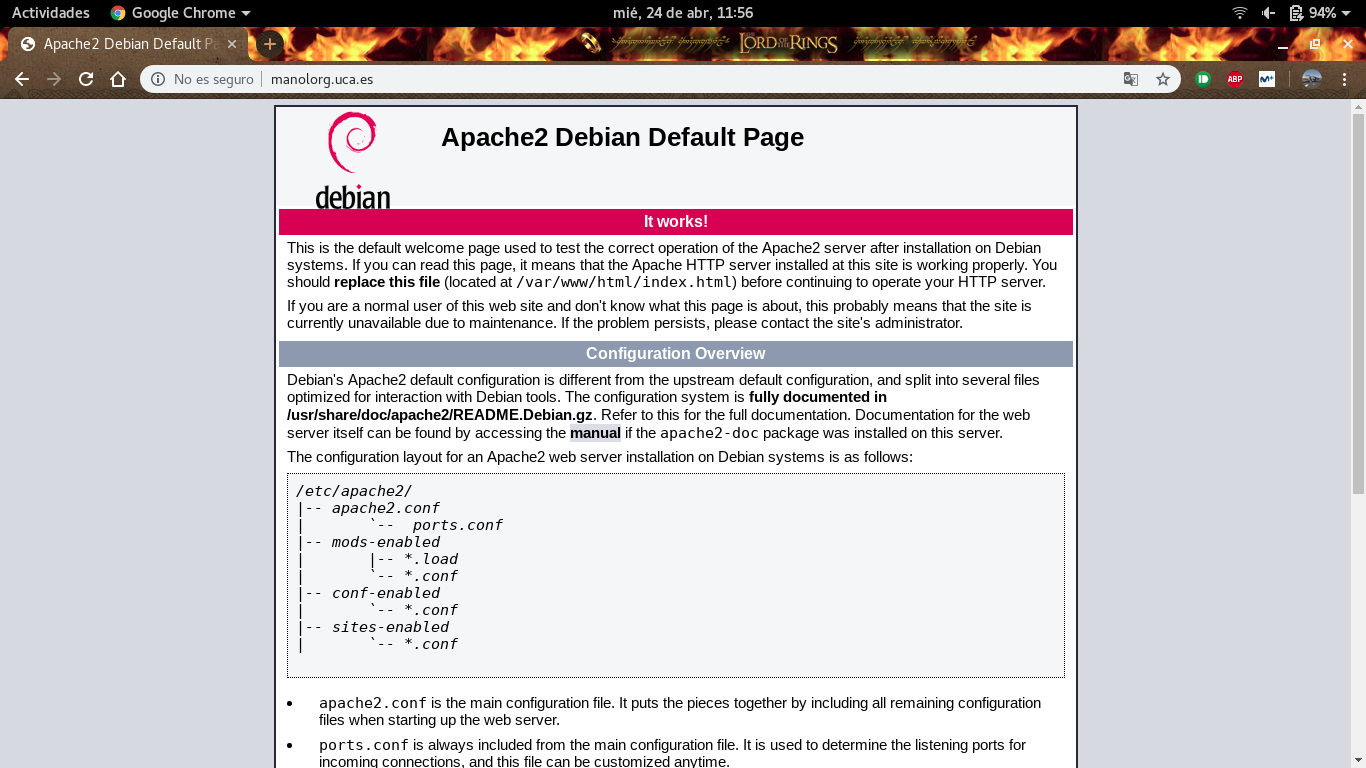
\includegraphics[scale=0.34]{Apache.png}
	\caption{Página inicial de Apache}
	\label{Página inicial de Apache}
\end{figure}

Para comprobar que Webmin está bien instalado, entramos en la siguiente dirección: 
\begin{center}
	\texttt{https://manolorg.uca.es:10000}
\end{center}
\begin{figure}[h]
	\centering
	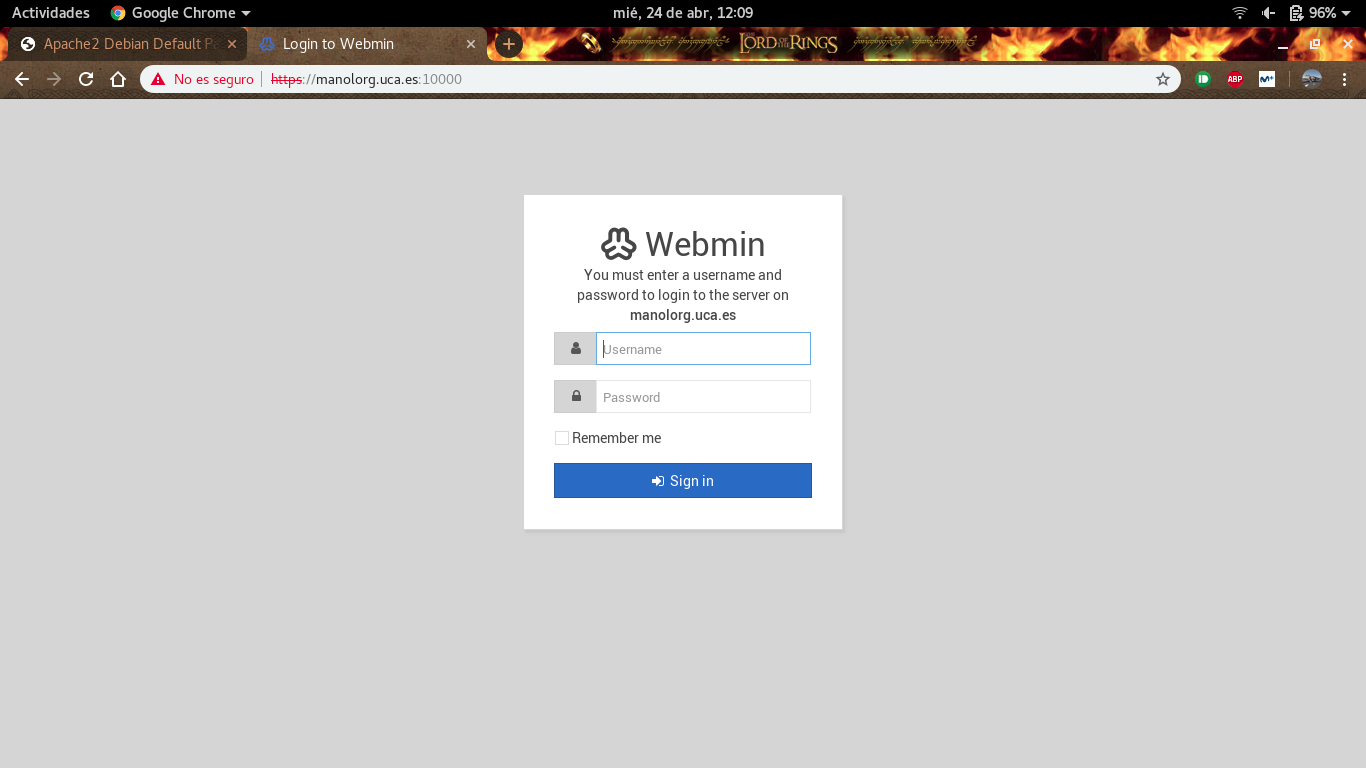
\includegraphics[scale=0.34]{Webmin.png}
	\caption{Página principal de Webmin}
	\label{Página principal de Webmin}
\end{figure}

\newpage
Para comprobar que php funciona bien cambiamos el archivo \texttt{/var/www/html/index.html} por \texttt{/var/www/html/index.php} y copiar el siguiente código en su interior:
\begin{lstlisting}[language=PHP]
<html>
  <head>
    <title>Prueba de PHP</title>
  </head>
  <body>
    <?php echo '<p>Hola Mundo</p>'; ?>
  </body>
</html>
\end{lstlisting}

Para ver si funciona, entramos en \texttt{manolorg.uca.es}.
\begin{figure}[h]
	\centering
	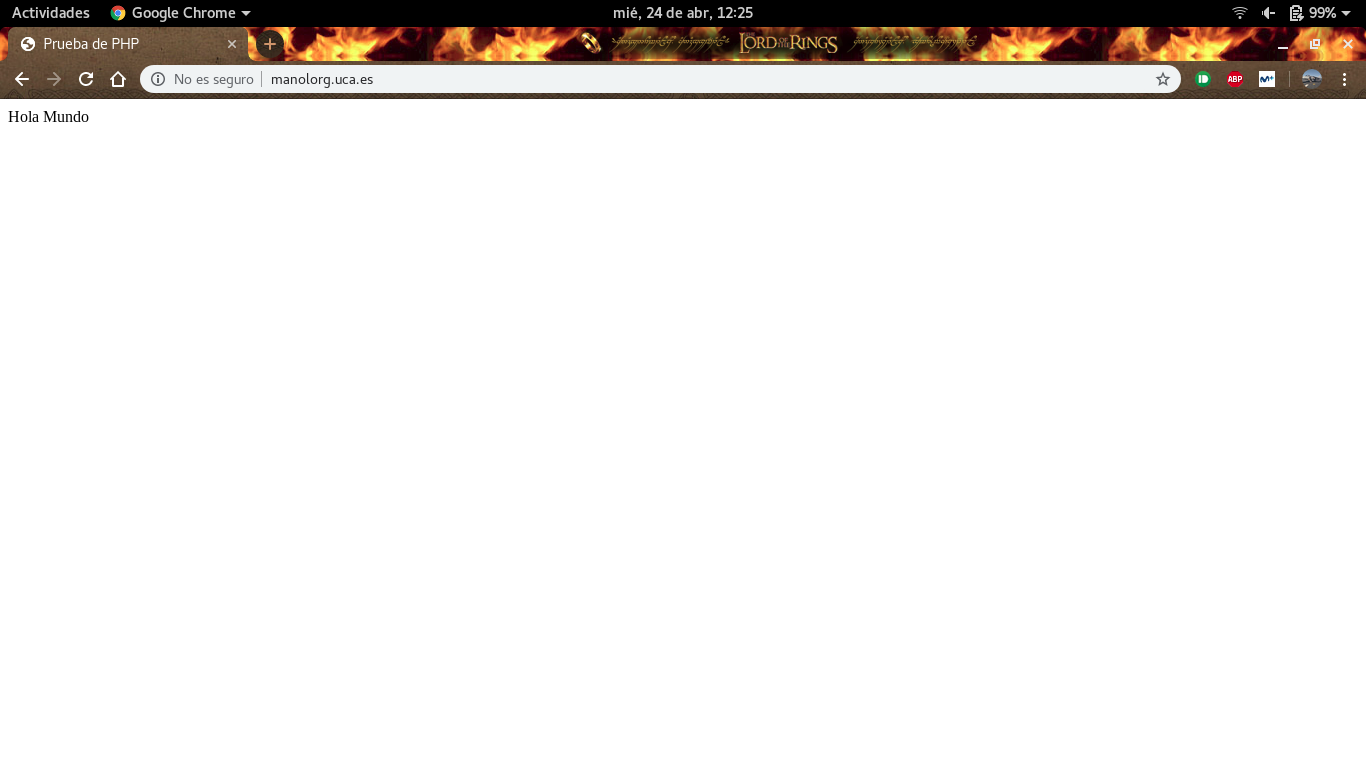
\includegraphics[scale=0.34]{PHP.png}
	\caption{Prueba PHP}
	\label{Prueba PHP}
\end{figure}

\newpage
\section{Configuración básica de apache}
Como ejemplo, vamos a modelar y configurar el entorno web del grupo de investigación Manolo Research Group.
\begin{itemize}
	\item La página principal del grupo está bajo el dominio \texttt{manolorg.uca.es}. El contenido se almacenará en \texttt{/var/www/manolorg}.
	
	Para ello accedemos a webmin y creamos un nuevo host virtual y, en document root ponemos \texttt{/var/www/manolorg}.
	
	\item Se desea que solo se acceda a la dirección \texttt{/docs} solo pueda acceder el usuario \texttt{admin} y el usuario \texttt{manolo}.
	
	\item No se mostrarán los directorios, excepto la carpeta \texttt{/software} que será solo accesible para el usuario \texttt{admin}.
	
	Para que el directorio \texttt{software} nos muestre el índice de archivos, tendremos que crear un nuevo ``directory'' llamado software, luego nos iremos al \texttt{Document Options} del nuevo directorio. Una vez ahí, tendremos que marcar la opción de ``Selected below'' y la opción ``Generate directory indexes'' como ``yes''. Quedaría como en la siguiente imagen:
	\newpage
	\begin{figure}[h]
		\centering
		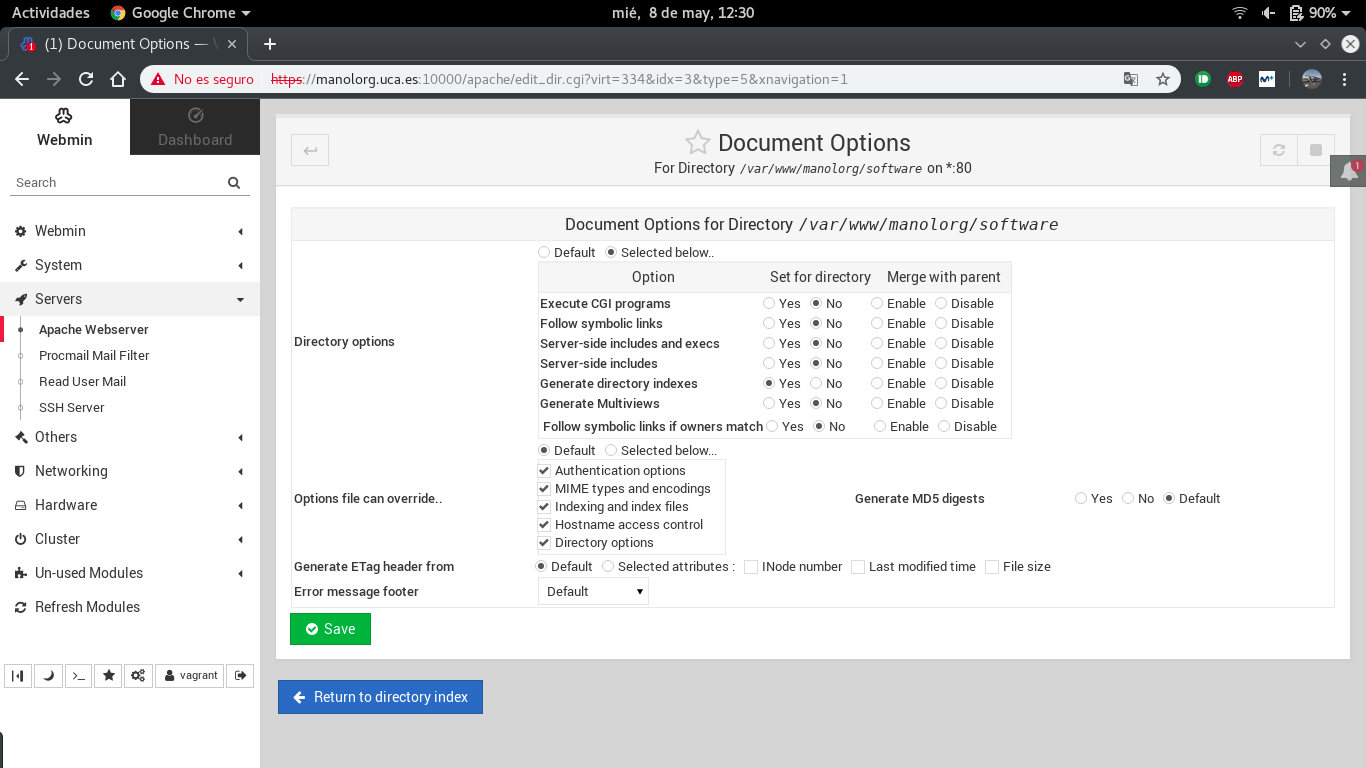
\includegraphics[scale=0.34]{Indexing.png}
		\caption{Document Options para software}
		\label{Document Options para software}
	\end{figure}
	
	\item La dirección \texttt{/sci2s} apuntará a la web \texttt{sci2s.ugr.es}.
	
	Para ello creamos el directory de \texttt{sci2s}, entramos dentro y le damos a ``Aliases and Redirects'' y ponemos la dirección deseada como en la siguiente imagen:
	\newpage
	\begin{figure}[h]
		\centering
		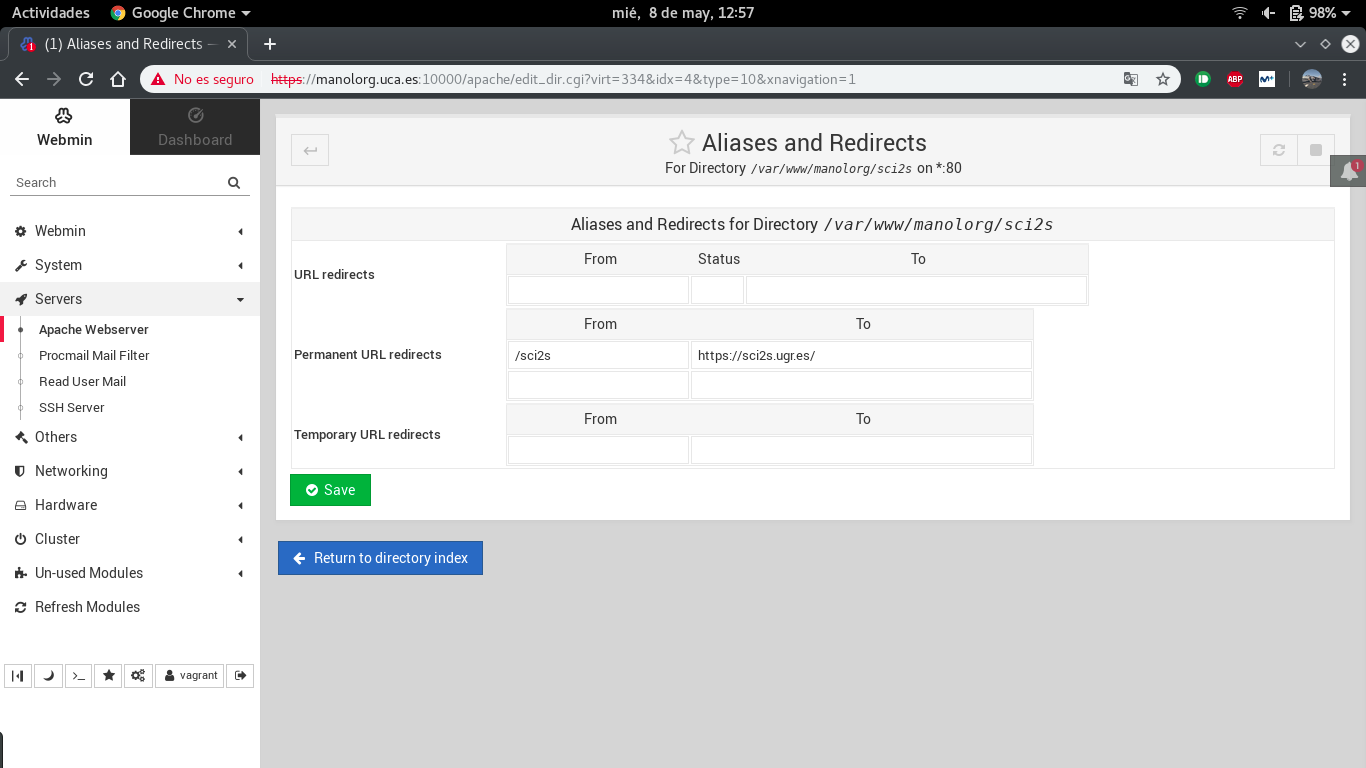
\includegraphics[scale=0.34]{ugr.png}
		\caption{Redirección a sci2s.ugr.es}
		\label{Redirección a sci2s.ugr.es}
	\end{figure}
	
	\item El grupo estará creado por diferentes laboratorios, crear un subdominio para el lab1 y el lab2. El contenido se almacenará en \texttt{/var/www/lab*}.
	
	Para ello, creamos dos carpetas nuevas desde la consola de la máquina virtual en \texttt{/var/www}, llamadas \texttt{lab1} y \texttt{lab2}.
	
	Para cada uno de los laboratorios, crearemos un virtual host distinto, y, en las opciones de creación, pondremos el document root en ``/var/www/labX'' (siendo X el número del laboratorio), pondremos el puerto 80, como \texttt{server name} pondremos ``labX.manolorg.uca.es'' (siendo X el número del laboratorio).
	
	PONER FOTO DE QUE CARGAN LOS LABORATORIOS
	
\end{itemize}

Se deberá crear una web sencilla (Hola mundo) en cada uno de los dominios y carpetas. Las páginas deben tener caracteres con tildes, por lo que debemos configurar Apache para que trabaje con UTF8.

Por defecto, no funciona la codificación UTF8, como podemos ver en la siguiente imagen:
\newpage
\begin{figure}[h]
	\centering
	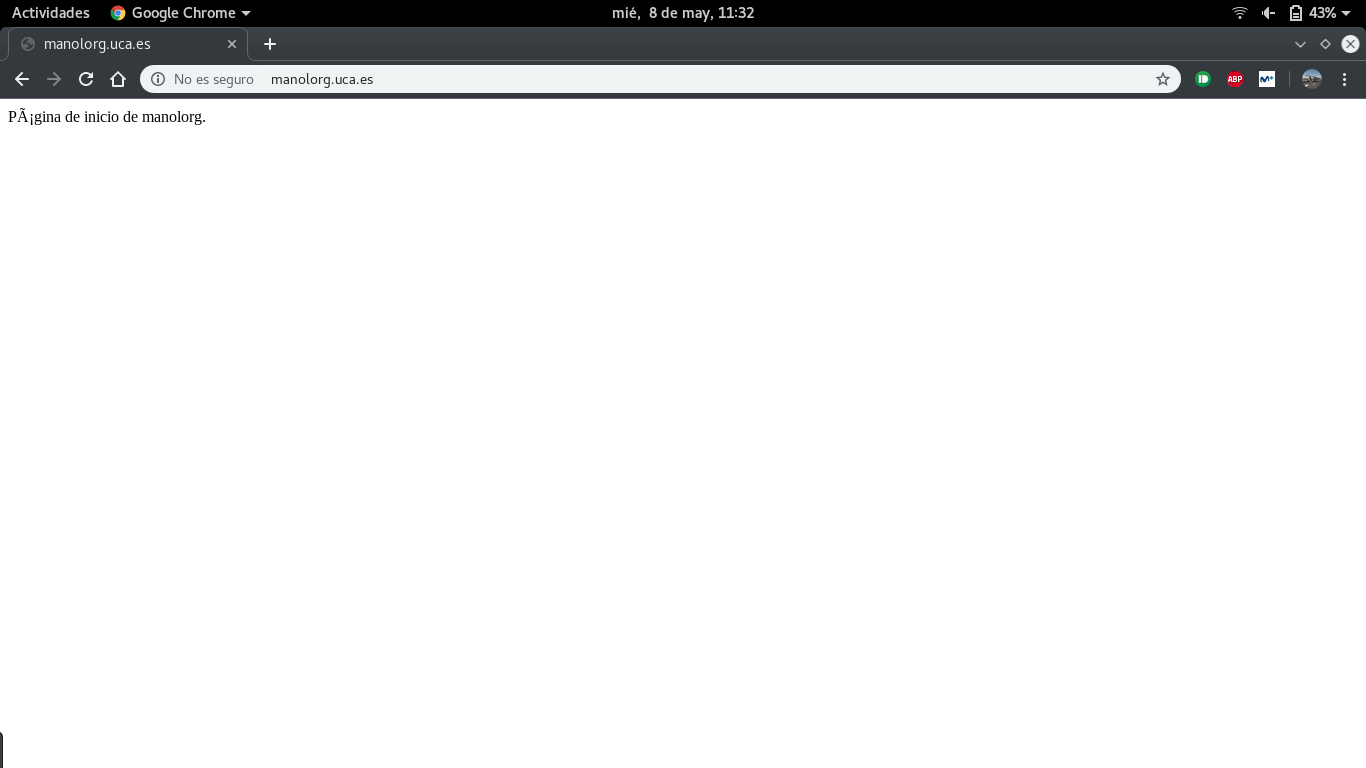
\includegraphics[scale=0.34]{SinUTF8.png}
	\caption{Sin UTF8}
	\label{Sin UTF8}
\end{figure}

Para activar el UTF8, nos dirigimos nos dirigimos a la edición de directivas globales (en la pestaña "global configuration") y añadimos la siguiente directiva al final\footnote{Si estamos usando Debian/Jessie debemos cambiar el archivo \texttt{/etc/apache2/conf-enabled/charset.conf} y descomentar la instrucción que dice: \texttt{\#AddDefaultCharset UTF-8}.}:
\begin{center}
	\texttt{adddefaultcharset utf-8}
\end{center}

\newpage
Una vez añadida la directiva mencionada, podemos ver como sí que funciona la codificación UTF8:
\begin{figure}[h]
	\centering
	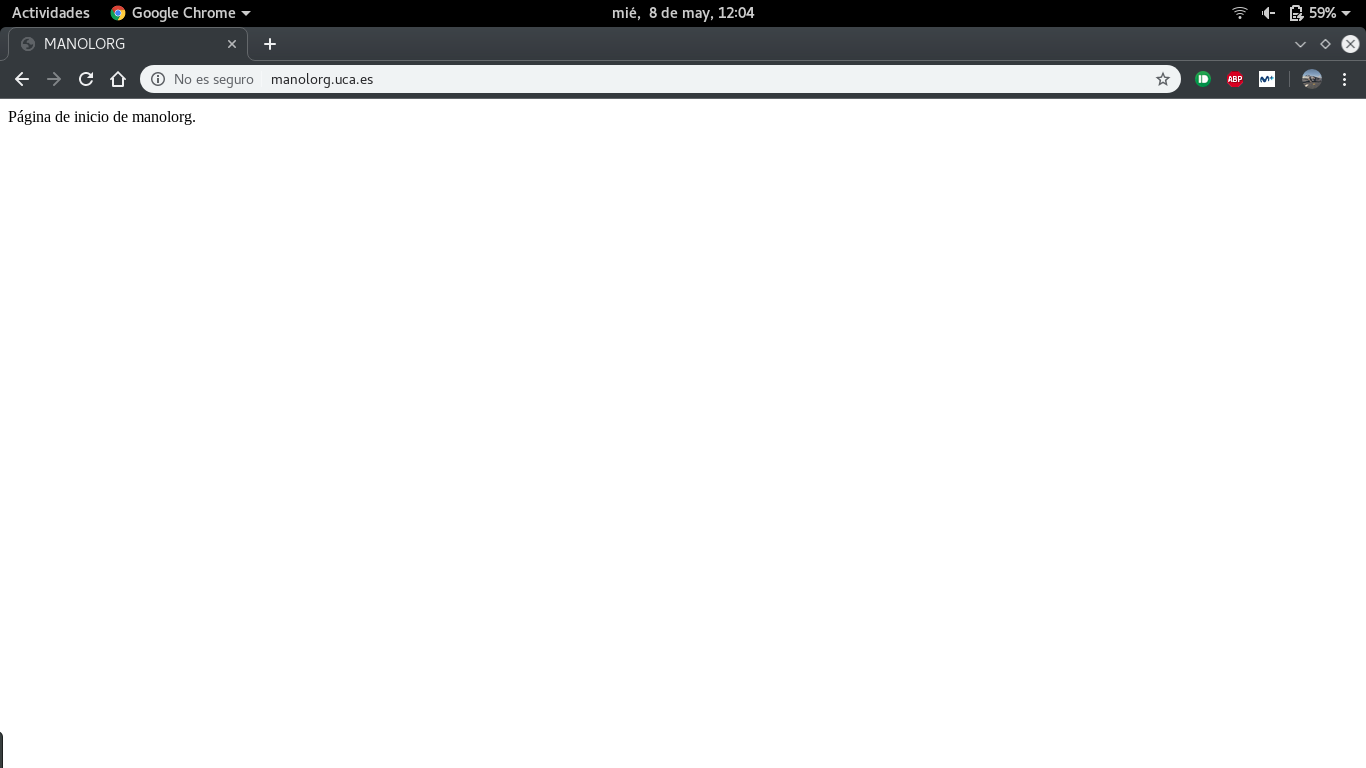
\includegraphics[scale=0.34]{ConUTF8.png}
	\caption{Con UTF8}
	\label{Con UTF8}
\end{figure}
\end{document}